\title{\vspace{-25mm}Sample Return Robot Challenge 2014 \\ Design Proposal}
\author{Team: RPIRR (Rensselaer Polytechnic Institute Rock Raiders)}
\date{\today}
\documentclass{paper}

%% Packages
\usepackage{algorithm}
\usepackage{algorithmic}
\usepackage{amsfonts}
\usepackage{amsmath}
\usepackage{bm}
\usepackage[labelfont=bf]{caption}
\usepackage{colortbl}
\usepackage{graphics}
\usepackage{graphicx}
\usepackage[ 	colorlinks = true,
            		linkcolor = blue,
            		urlcolor  = blue,
            		citecolor = blue,
           		anchorcolor = blue]{hyperref}
\usepackage{pifont}
\usepackage{setspace}
\usepackage{sidecap}
\usepackage{subcaption}
\usepackage{tikz}
\usetikzlibrary{arrows,fadings,positioning,shapes,snakes}
\usepackage{titlesec}
\usepackage{url}
\usepackage{wrapfig}
\usepackage{xcolor}



%% Useful commands
\newcommand{\tab}{\hspace*{2em}}
\newcommand \todo[1]{\textcolor{red}{[#1]}}
\newcommand \robotName{Rockie} 		% Edit here to change robot name


%%%%%%%%%%%%%%%%%%%%%%%%%%%%%%%%%%%%%%%%%%%%%%%%%%
\begin{document}
\maketitle


%%%%%%%%%%%%%%%%%%
% Overview
\section*{Overview of design}

	This document contains a brief overview of our design goals as well as relevant descriptions of materials and preliminary design choices.  As this is our first year participating, we will be trying to keep our design straight forward.  ``\robotName" will be a four-wheeled mobile robot with scoop and rake.  Objects will all be stored in the hull, separated by cloth or plastic dividers.   An on board computer running ROS will control the autonomous sensing, roving, and object acquisition.   
%attached to a 3-DOF arm, bins for separating retrieved objects, multiple cameras, and autonomous controls built in ROS.  

\begin{figure}[htp]
\centering
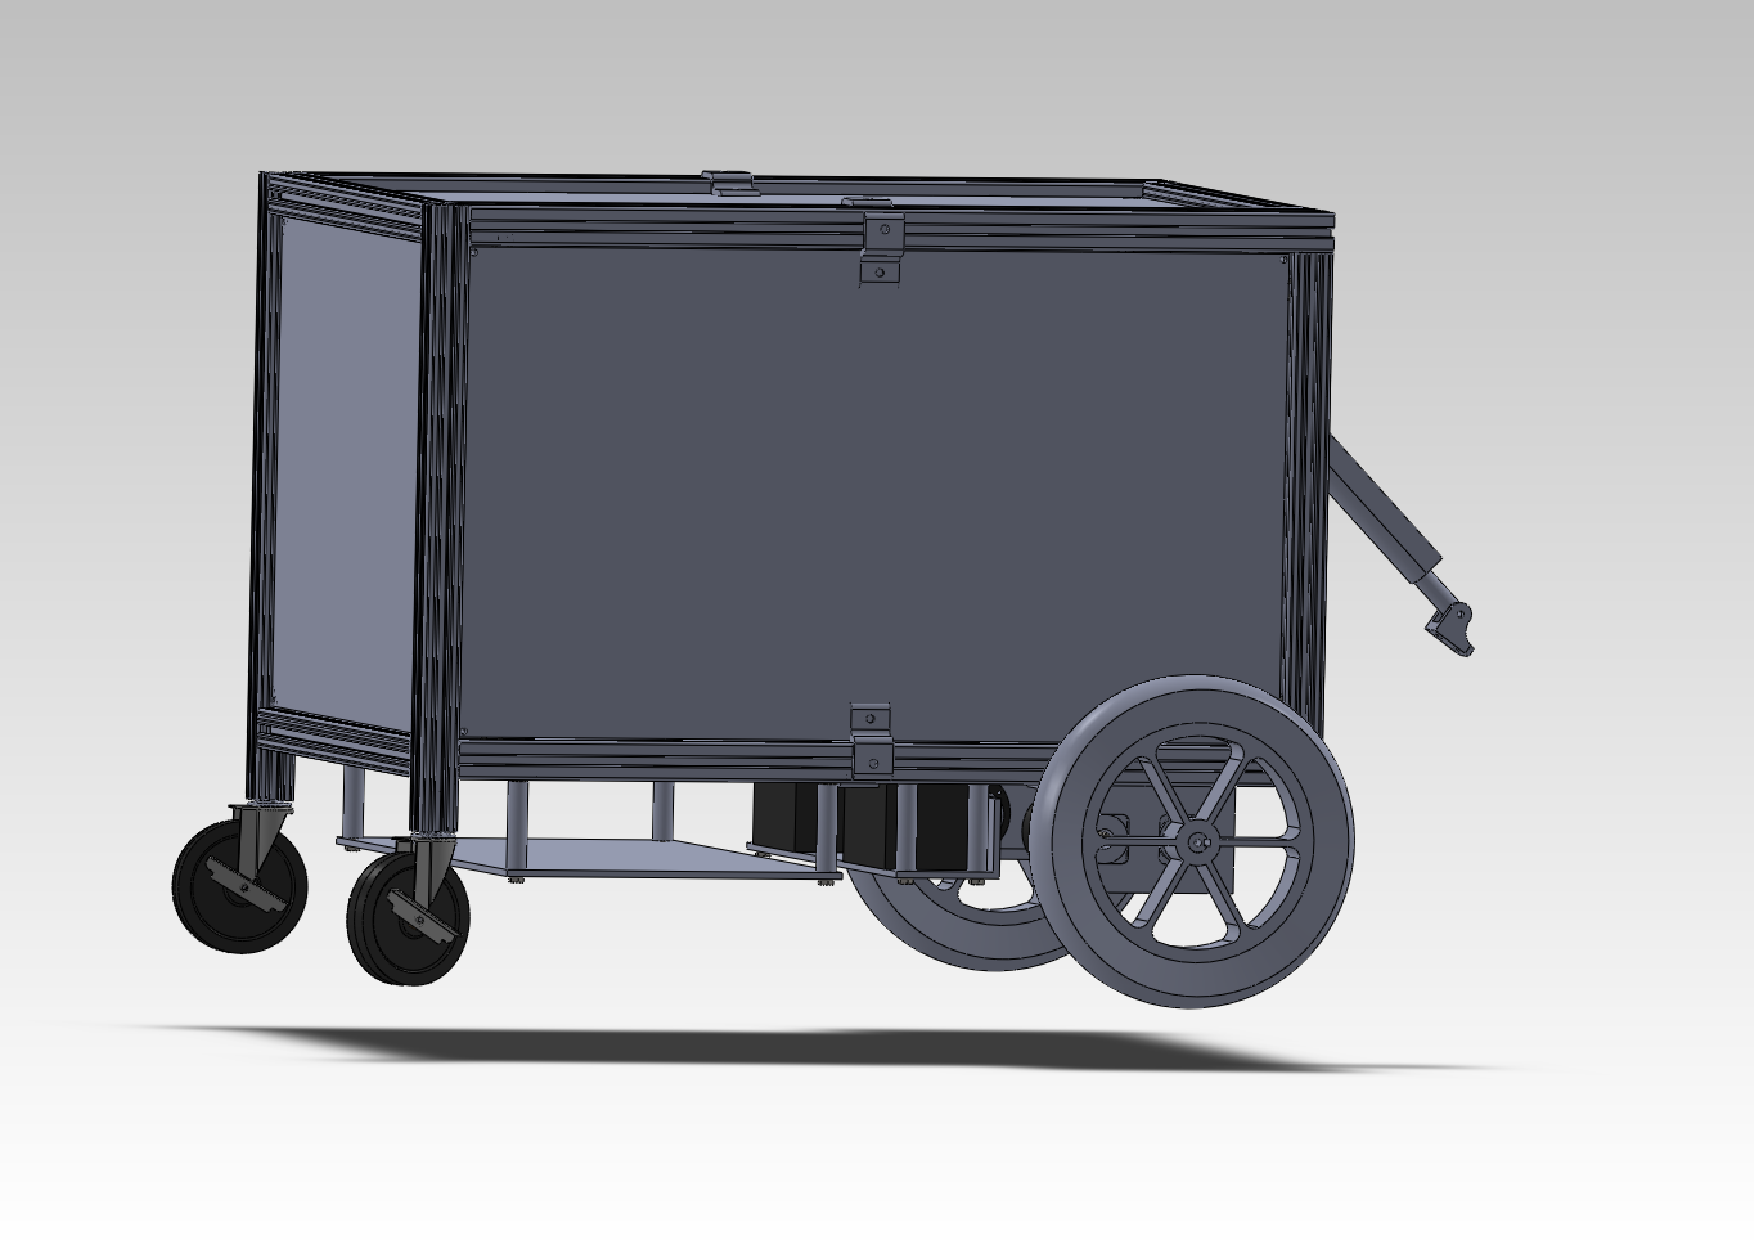
\includegraphics[width=0.65\textwidth]{fig/robot_assembly_1.PDF} \\ 
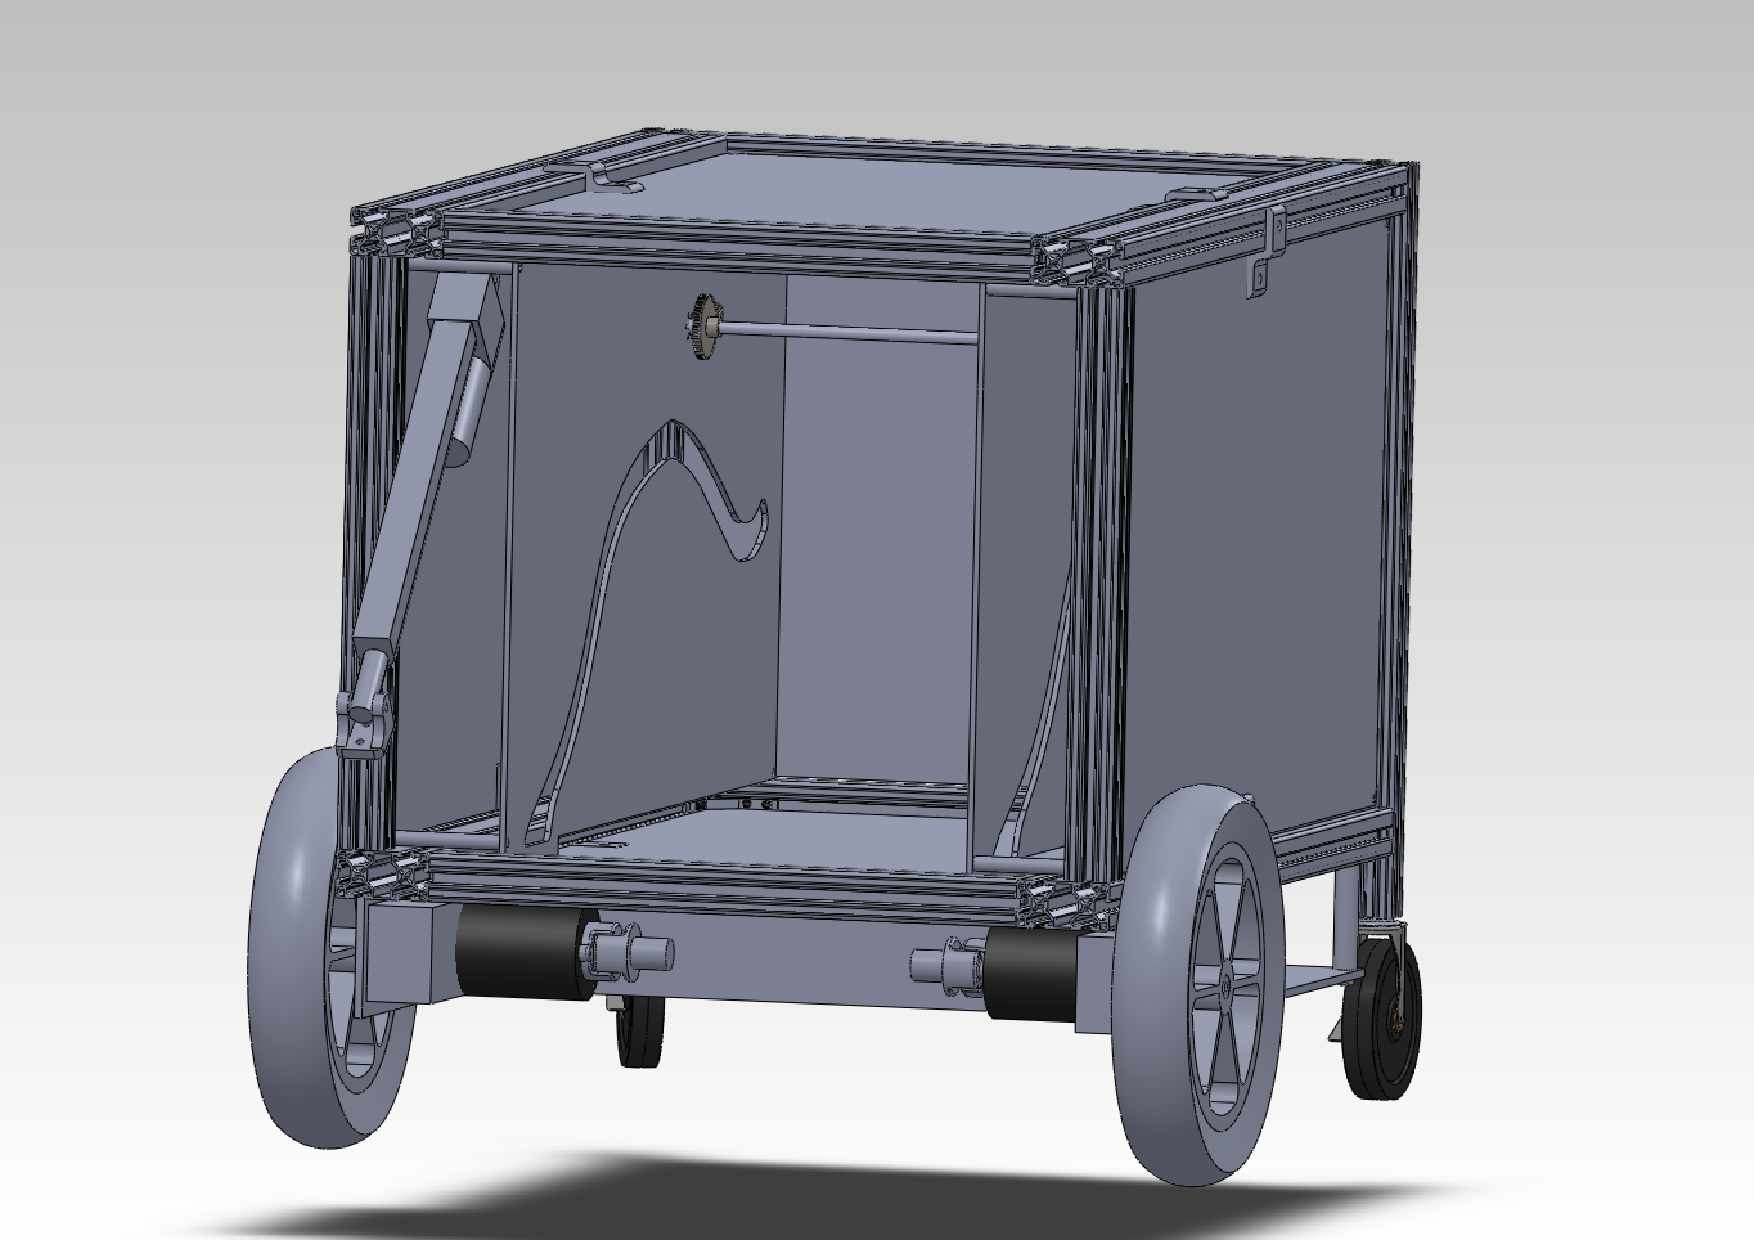
\includegraphics[width=0.65\textwidth]{fig/robot_assembly_2.PDF} \\
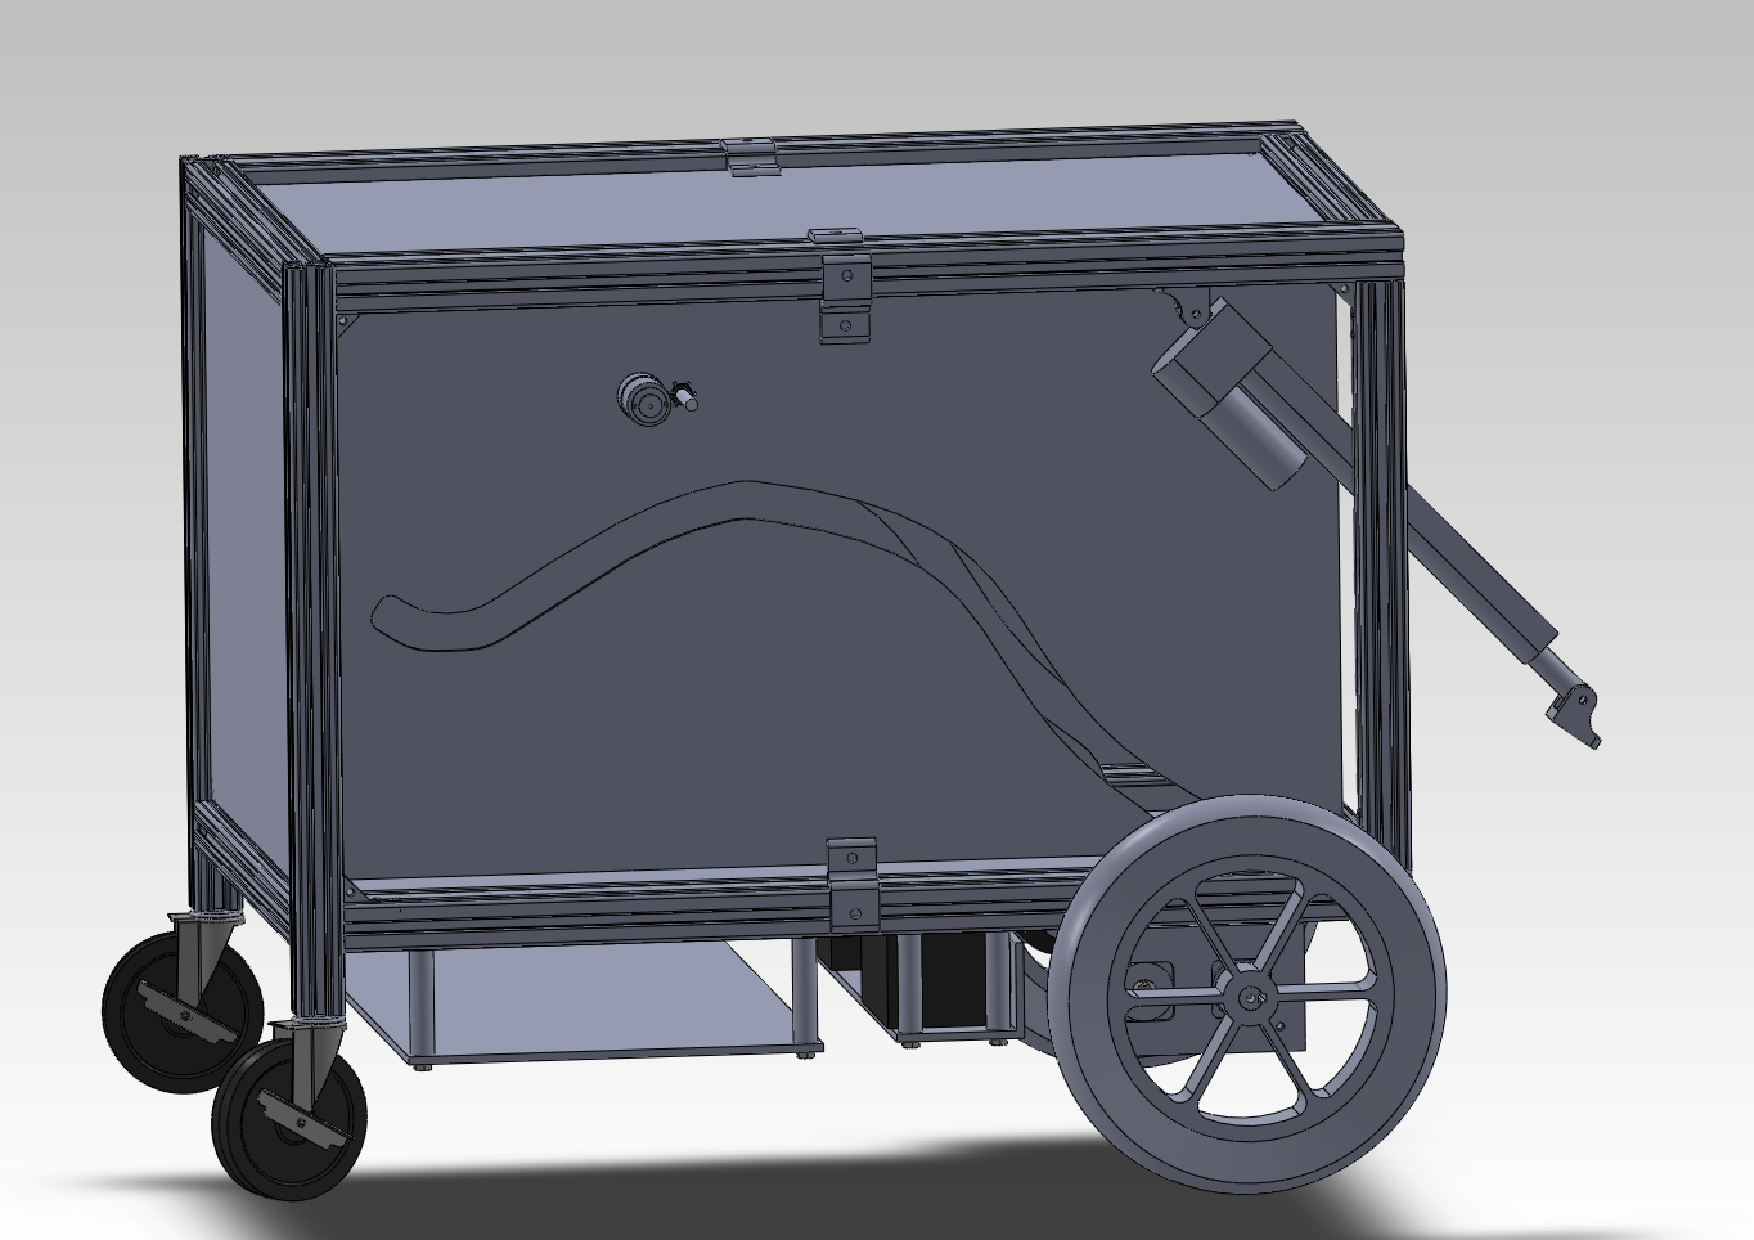
\includegraphics[width=0.65\textwidth]{fig/robot_assembly_3.PDF}
\caption{A sketchup of \robotName. }
\label{fig:sketchup}
\end{figure}

%%%%%%%%%%%%%%%%%
\subsection*{Detailed Description of Approach}

	Upon startup, \robotName \ will scan surrounding area in attempt to triangulate position with respect to given features.  If unsuccessful, \robotName \ will traverse the course in a manner to expand its map, until a tranform between its map and given map is formed.  Upon success, it will travel to precached object, continuing to generate a more detailed map and noting possible samples.  Upon arriving at precached approximate location, it will do an expanding search until locating the sample.  Using stereo vision, it will use depth location to navigate within range of the object.  Then it will lower its scoop, with the rake extended.  Upon verifying object within bounding box of the rake and scoop, the rake will retract, pulling the sample onto the scoop.  Once verified the sample is on the scoop, the scoop will be raised, dropping the object into the robot, onto a cloth sheet.  Verifying the object is within the robot, a motor will raise the sheet, pulling the object further into the robot and creating a barrier between it and further objects.  Keeping track of time, the robot will further explore the area, furthering it boundaries, searching for possible samples.  \robotName \ will explore possible candidates and correct as described above.  Once time becomes an issue, it will return to the platform using its map and a homing beacon of a large easily identified image. 

%%%%%%%%%%%
\subsection*{Hardware and electronics}

	% Communication protocols and frequencies used.
	The only communication we will implement is a wireless pause switch.  For this, we will use an XBee PRO at 2.4 GHz, since it has excellent range and is easy to use.

	% Sensors for localization, navigation, obstacle avoidance, and sample id
	\robotName\text{ }will be equipped with at least two cameras: 
\begin{itemize}
	\item A stereo camera mounted near the front of the robot with 2 DOF, pan and tilt, for SLAM and object recognition.
	\item A webcam for object and capture verification
	%\item A low-definition camera mounted near the gripper for use during grasping.
\end{itemize}
All cameras will be able to contribute to object and sample identification.  
	Navigation, including localization and obstacle avoidance, will involve the very popular SLAM approach.  In particular, we will utilize the rgbdslam ROS package.  

In addition to cameras, \robotName \ will have 2 Hokuyo LIDAR (URG-04LX-UG01) for navigation.


%%%%%%%%%%%
% Electronics
	The following is a list of electronic components we will use in addition to the cameras:
\begin{itemize}
	\item Laptop running ROS
	\item 2x geared 12V DC motors for driving
  \item Sabertooth Dual 60A 6-30V Regenerative motor driver for drive motors
  \item 2x 12V linear actuators with L298N H-bridges
  \item geared 12V DC motor for folder system with L298N H-bridges
	\item Arduino as motor controller
	\item Deep-cycle lead-acid battery and voltage regulator
\end{itemize}


\begin{figure}[htp]
\centering

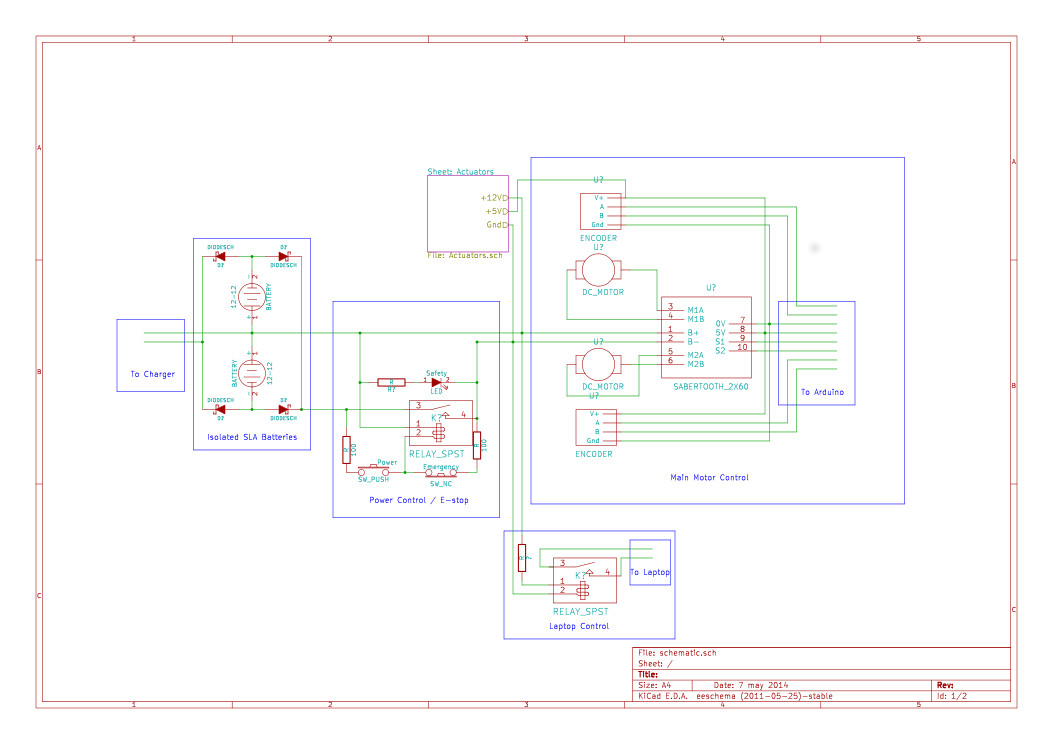
\includegraphics[width=0.95\textwidth]{fig/schematic.jpg}


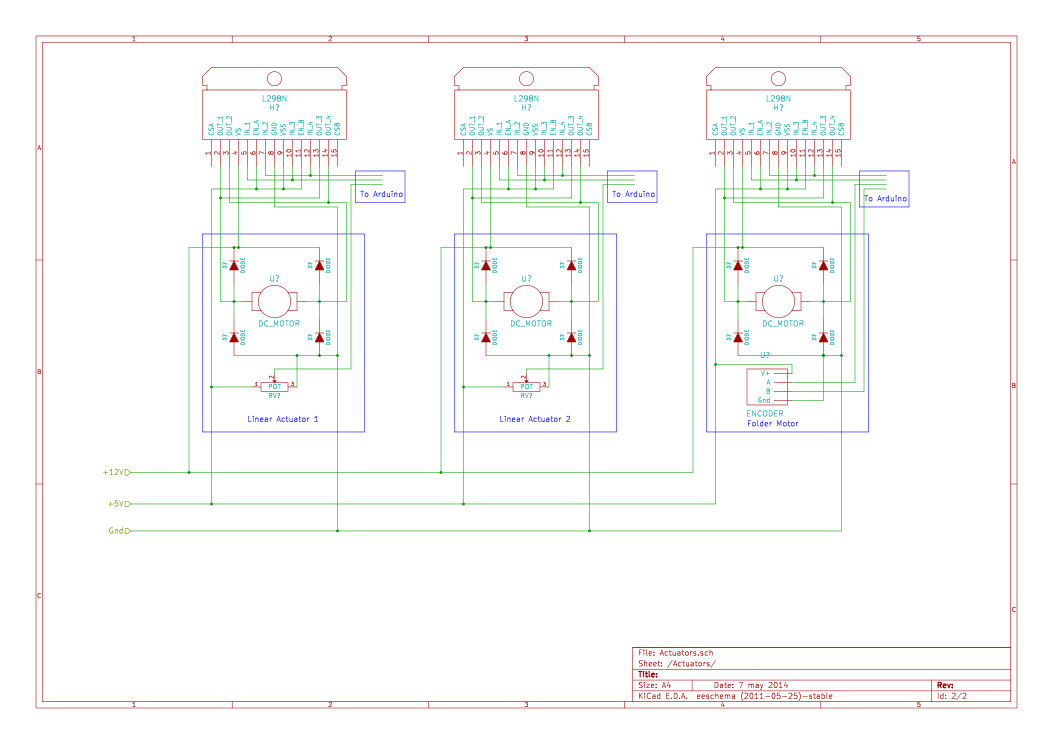
\includegraphics[width=0.95\textwidth]{fig/schematic-Actuators.jpg} 
\caption{Circuit diagram of \robotName}
\label{fig:sch}
\end{figure}



%%%%%%%%%%%
\subsection*{Safety features}

	% Wireless kill switch / on-board E-Stop
	\robotName \ will have a master power switch, mechanical e-stop (see circuit drawing Figure 2), and wireless pause switch in accordance with rules R18 and R19.  The pause switch will be a simple remote switch that sends a message over xbee to stop all moving parts, with the exception of a built in cooling fan on the sabertooth motor driver.  \robotName \ will also have a safety light to display its state.  
	% Hazardous materials compliance (battery?)
	\robotName \ will contain no hazardous materials as per rule R17.  



%%%%%%%%%%%
\subsection*{Software}

	We will use ROS as our software platform since it offers many useful libraries, in particular SLAM, SIFT, and PCL to name a few.     

\subsubsection*{Object identification using OpenCV and ROS}
The open-source vision package OpenCV has been around for a long time and there are many available algorithms that we could take advantage to identify the ``samples" that we want to pick up. Since  our software platform is Robotics Operating System (ROS), we need to set up the interface between ROS and OpenCV. The output from the tracking system provides important information for the SLAM and navigation. \\ 

The following is a high-level flow chart of how the nodes communicate using topics. The blue rectangles are the nodes while the red ellipses are the topics. The arrow is pointing to the node, which subscribes to the topic. 

% Define block styles
%\tikzstyle{decision} = [diamond, draw, fill=red!20, 
%    text badly centered, node distance=3cm, inner sep=0pt]
\tikzstyle{block} = [rectangle, draw, fill=blue!20, 
     text centered, rounded corners, minimum height=3em]
\tikzstyle{line} = [draw, -latex']
\tikzstyle{cloud} = [draw, ellipse,fill=red!20, node distance=3cm,
    minimum height=2em]
\begin{tikzpicture}[auto]
    % Place nodes
    \node [block]  (camera)  at (0, 0) {rockie\_camera\_node};
    \node [block]  (imageproc) at (10, 0) {image\_process\_node};
    \node [block]  (postproc) at (10, -4) {post\_processing\_node};
    \node [block]  (navigation) at (0, -4) {navigation\_node};
    \node [block]  (scoop)     at (0, -7) {scoop\_node};
    \path [line]   (camera) -- (imageproc);
    \path [line] (imageproc) -- (postproc);
    \path [line] (postproc) -- (navigation);
    \path [line, dashed] (navigation) -- (camera);
    \node [cloud] (rawimg) at (5, 0.4) {/camera/image\_raw};
    \node [cloud] (procimg) at (10, -2) {/camera/image\_processed};
    \node [cloud] (sample) at (5, -4) {/is\_sample};
    \node [cloud, dotted] (capture) at (0, -2) {/take\_pictures};
    \path [line]  (sample) -- (scoop);
\end{tikzpicture}
We are using the Logitech $C920$ camera. Once the camera takes a picture, the frame will be published as a topic ``\/camera\/image\_raw". 
Since the ``image\_process\_node" subscribes to this topic, once the raw\_image is published, it will be processed inside ``image\_process\_node" and a new topic ``\/camera\/image\_processed" is published for post processing. Here it is worth to mention that the OpenCV feature detection algorithms are used in the ``image\_process\_node". After the post processing, the robot is confident whether the object is an sample and decides whether or not to pick it up.   

The following are some initial object matching results using combination of ROS and OpenCV package: 
\begin{figure}[htp]
\centering
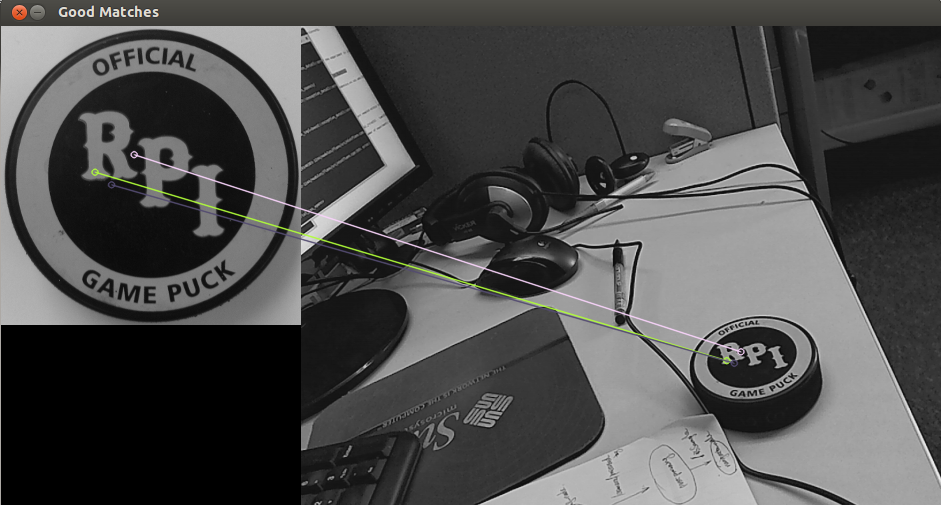
\includegraphics[width=0.95\textwidth]{fig/vision1.png}  

 
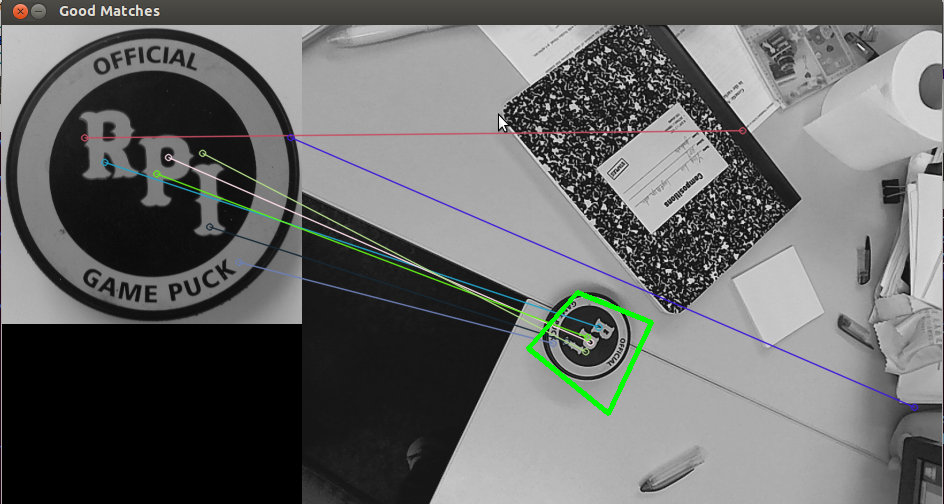
\includegraphics[width=0.95\textwidth]{fig/vision2.png} 

 
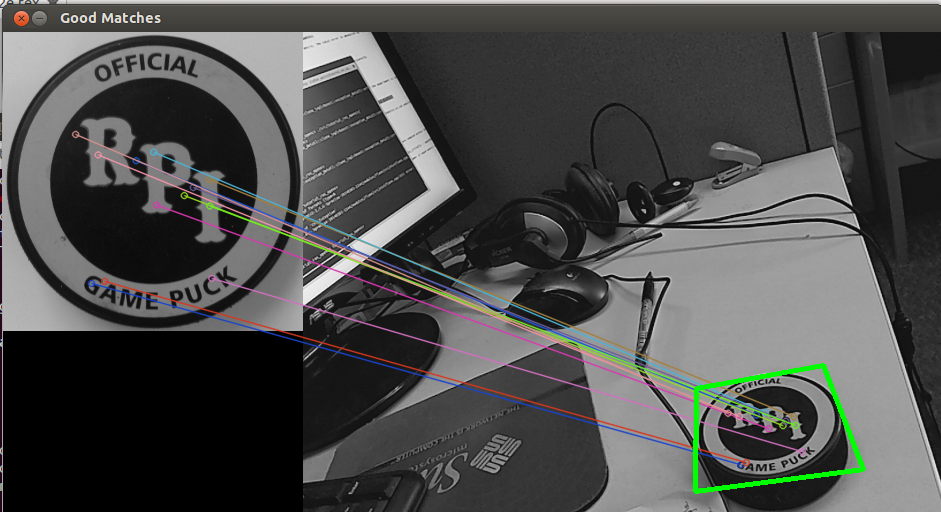
\includegraphics[width=0.95\textwidth]{fig/vision3.png}
\caption{The left picture is a puck image cached in database, the right one is taken from the web camera.}
\label{fig:vision}
\end{figure}
Thick green square means the algorithm is confident to find the cached object in the active frame, while the lines shows the matching between the cached image and the picture from the live frame. Right now this object identification testing is limited to feature and geometry. Colour detection will be added to the package.

\subsubsection*{Navigation}
Most navigation will be done using existing ROS packages.  SLAM will be done using RGBD-SLAM package.  The map will be flattened to 2D with obstacles generated for navigation purposes.  \robotName \ navigates with the ROS navigation stack.  Odometry will be gathered with the visual odometry package viso2.  Motor control is done on the arduino with PD velocity controller using encorder values of the motor.

\section*{Future Work}
There is a great amount of work we would still like to do before the competition.

\subsection*{Hardware}
In hardware, we need to finish the rake and attach it to the scoop.  A first level rake has been designed and implemented, but due to miscommunication leading to delayed parts, the is unattachable.  In addition, there are some improvements we would like to the initial rake for more secure object capture.  Related, we would like to make the scoop a little more rigid and add some basic features for more robust object capture.

The next task in hardware is mounting the sensors.  The stereo camera system will be self built, but has yet to be finished.  Additionally the extra cameras and lidar system mounts have yet to be built.  Also the final electronic mounts need to be completed.

The folder system, while designed, needs to be built.

\subsection*{Electronics}
While most circuits are designed, some still need to be wired.  In addition, the laptop power needs to be integrated with the E-stop as stated in the design.

The pause controller needs to be built and the related circuits.

\subsection*{Software}
The code for exploring and expanding the map has yet to be implemented.  In addition the code for approaching the object and capturing it has yet to be written.

The executative code that runs the system is a system state machine.  This code has been started, but needs to be finished.  As part of this, the different code parts need to be integrated together, as many of them are still separate.

Further, while we have moderate object recognition software, we hope to improve it to be more robust, precise, and accurate.

\end{document}

